% v2-acmtog-sample.tex, dated March 7 2012
% This is a sample file for ACM Transactions on Graphics
%
% Compilation using 'acmtog.cls' - version 1.2 (March 2012), Aptara Inc.
% (c) 2010 Association for Computing Machinery (ACM)
%
% Questions/Suggestions/Feedback should be addressed to => "acmtexsupport@aptaracorp.com".
% Users can also go through the FAQs available on the journal's submission webpage.
%
% Steps to compile: latex, bibtex, latex latex
%
% For tracking purposes => this is v1.2 - March 2012
% you may choose between british, american and german as an language option
% logo options are: hcilogo, uwblogo, no logo (no option means default logo)
\documentclass[american]{acmtog} % V1.2
\pagenumbering{arabic}
% Farbdefinitionen fuer Hyperref (s.u.) und Tabellen
\usepackage[table, svgnames]{xcolor}

\definecolor{dkblue}{RGB}{0,0,128}
\definecolor{dkorange}{RGB}{255,128,0}
\definecolor{purple}{RGB}{102,14,122}
\definecolor{ontology}{RGB}{0,128,255}
\definecolor{groundedsymbols}{RGB}{128,69,0}
\definecolor{string}{RGB}{0,128,0}
\definecolor{type}{RGB}{32,153,157}
\definecolor{comment}{RGB}{128,128,128}
\definecolor{comment}{RGB}{128,128,128}
\definecolor{real}{RGB}{0,0,255}
\definecolor{gray}{RGB}{128,128,128}
\definecolor{cps}{RGB}{128,128,0}
\usepackage[unicode=true, breaklinks=true, colorlinks=true]{hyperref}
\usepackage{enumitem}
\usepackage{float}
\hypersetup{%
citecolor=dkblue,
urlcolor=dkorange,
linkcolor=dkorange
}

\addbibresource{VATRY_literature.bib}

\documentTitle{Head's Oscillations Simulation - Project Report} 
\documentMonth{July}
\documentYear{2024}

\documentAuthor{Etienne VATRY}

\projectType{HCI Project Report supervised by\\Jean-Luc LUGRIN}

\begin{document}
\pagenumbering{gobble}

\maketitle

\begin{bottomstuff}
etienne.vatry@stud-mail.uni-wuerzburg.de
\end{bottomstuff}

\begin{abstract}
ABSRACT Cybersickness is an obstacle to the development of virtual reality applications in any field. If the user experience is negative due to discomfort, it will hinder the adoption and advancement of virtual reality technologies. This can even have critical effects, for example in medical applications. Through this project, we aim to set up a system that will enable us to measure the impact, positive or otherwise, of simulating head oscillations during user movements. More specifically, we will be focusing on oscillations during walking or running. For this purpose, three virtual environments have been set up, with three different types of terrain. Tests can be carried out regularly to measure the user's discomfort in real time.
\end{abstract}


\section{Introduction}
\label{sec:introduction}
The aim of this project was to create three virtual environments for virtual reality testing. The three environments are as follows:
\begin{itemize}[label=\textbullet]
    \item Flat terrain,
    \item Terrain with regular bumps,
    \item Terrain with noise-generated bumps.
\end{itemize}
At present, these lots are empty: they have no vegetation.

\begin{figure}[H]
\centerline{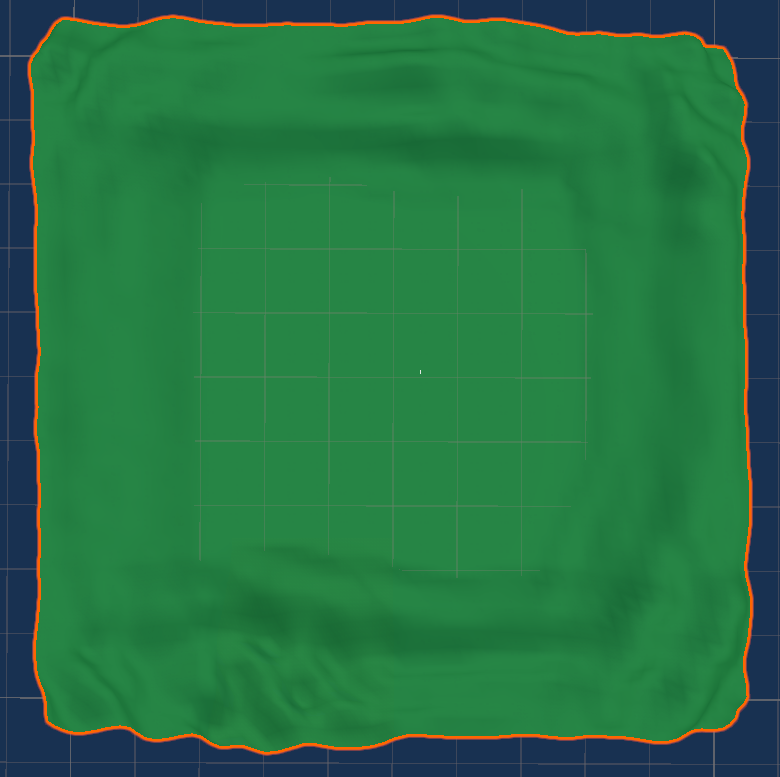
\includegraphics[width=\columnwidth]{figures/terrain.png}}
\caption{Terrain from above.}
    \label{fig:terrain}
\end{figure}

\begin{figure}[H]
\centerline{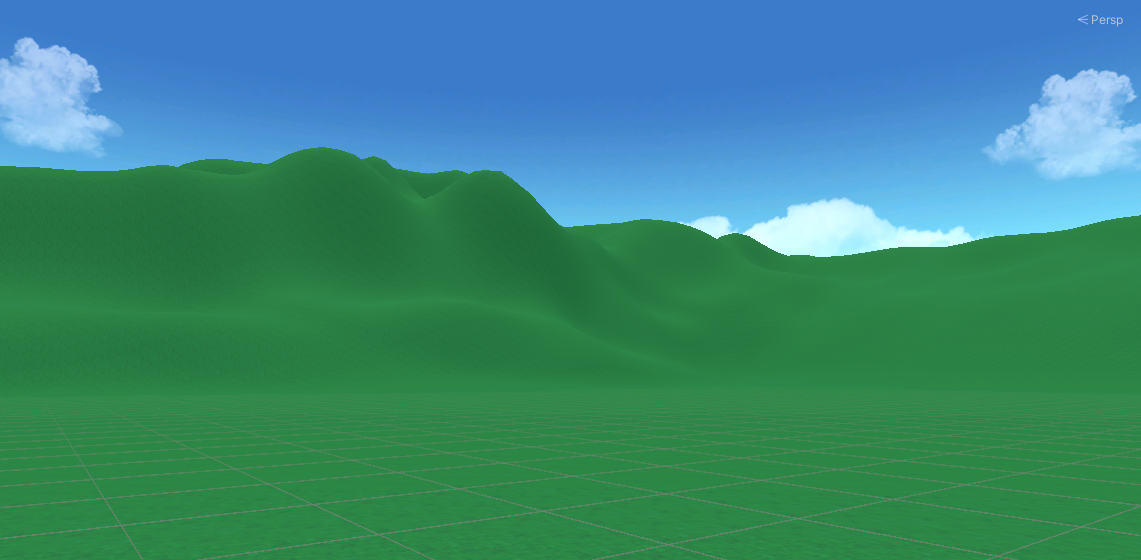
\includegraphics[width=\columnwidth]{figures/montains.png}}
\caption{Montains surrounding the terrain.}
    \label{fig:mountains}
\end{figure}

However, they have all been designed on the same basis - a large, flat surface surrounded by mountains. The choice to have three different terrains was motivated by a study showing that the more irregular the terrain, the greater the visual discomfort [\cite{bumpy_ride}]. It may therefore be interesting to observe how this discomfort evolves with the addition of head oscillations. During a simulation, Fast Motion Sickness scales can be used at regular intervals to monitor the user's condition in real time. Step sounds have also been added. These sounds have also been shown to reduce cybersickness [\cite{audio_in_vr},\cite{walking_vibe}]. Finally, the user's head oscillations during movement can be activated or deactivated, allowing the difference in user experience to be highlighted.

\section{Design and Development}
\label{sec:design}
\subsection{Tools and Technologies}
\subsubsection{Unity Engine}
To create these different virtual environments, we used Unity Engine. This choice was motivated by the flexibility of this tool, the presence of already complete templates, the wide variety of packages available, as well as its popularity. This popularity guarantees the availability of numerous resources and an active online community.

\subsubsection{Other Tools}
C\# has been chosen as the programming language for the various scripts. This is the language used by default on Unity. Sounds are in wav files.

\subsection{Methodology}

\subsubsection{Research and Planning}
The first part of this project focused on two main points:
\begin{itemize}[label=\textbullet]
    \item Getting to grips with Unity Engine,
    \item Various research studies.
\end{itemize}
These steps gave me an initial idea of what needed to be done during the project. At the end of these two stages, a first provisional schedule was created (see Figure \ref{fig:planning}). Its aim was to be as realistic as possible to ensure steady progress in the project. In addition, bi-monthly meetings were organized to avoid the tunnel effect and understand how to improve the project.

\begin{figure}[H]
\centerline{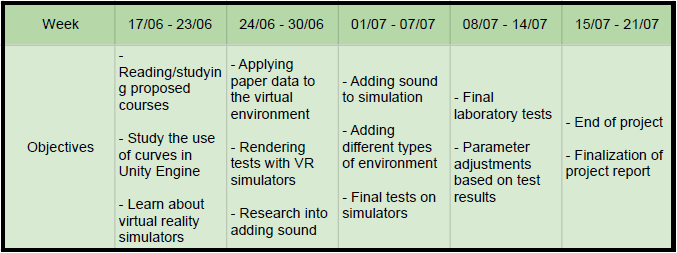
\includegraphics[width=\columnwidth]{figures/Planning.png}}
\caption{Initial project schedule.}
    \label{fig:planning}
\end{figure}

\subsubsection{Development Process}
Once the schedule was established, the project could begin. The idea was as follows: first of all, we wanted to have a simulation that worked without virtual reality, so that we could fully understand how it worked. We therefore worked on the virtual environment with the flat terrain, the other two terrains being copies of the latter with added relief. The steps were as follows:
\begin{itemize}[label=\textbullet]
    \item Creating the environment,
    \item Add displacements,
    \item Adding oscillations,
    \item Add tests during simulation,
    \item Adding step noises.
\end{itemize}
Secondly, we had to adapt this to virtual reality. We therefore had to change the camera and movement controls. The rest remained more or less unchanged.

\subsection{Environment Design}
As described in the introduction (\ref{sec:introduction}), the terrain was created from a research paper [\cite{bumpy_ride}]. The bumps of the second and third terrains are generated when the simulation is launched, enabling the parameters to be modified before the simulation begins. The three sections below describe these different environments in greater detail:

\subsubsection{Flat Terrain}
This terrain serves as the basis for the design of the other two. Apart from the mountains surrounding the surface where the user can evolve, there is no relief.

\subsubsection{Terrain with Regular Bumps}
For this terrain, regular linear bumps have been added at regular intervals. Their height and spacing can be modified to test different types of bump.

\begin{figure}[H]
\centerline{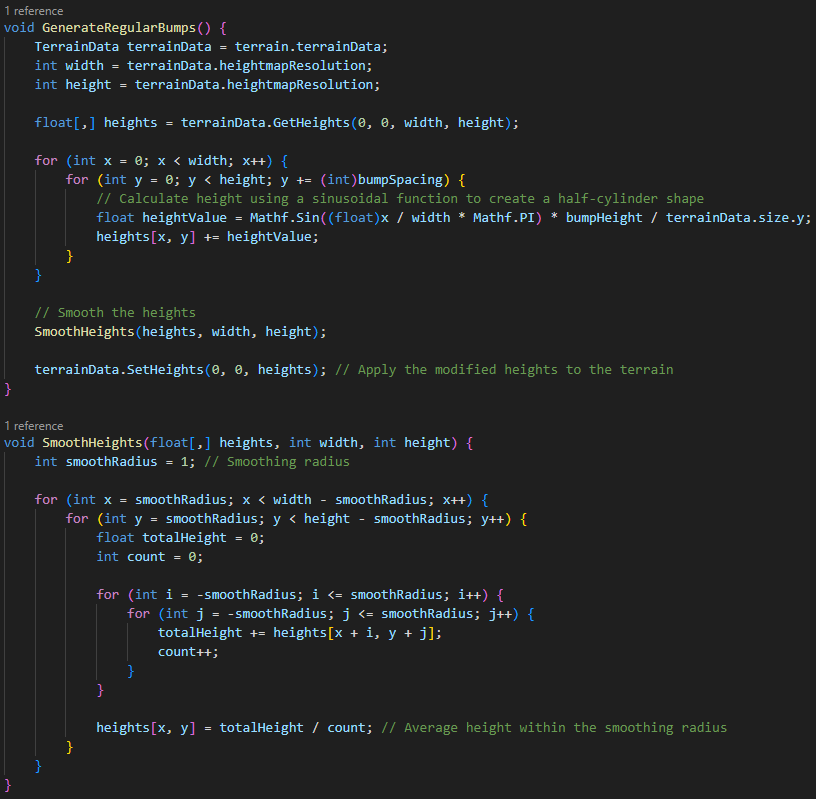
\includegraphics[width=\columnwidth]{figures/regular_bumps_code.png}}
\caption{Regular bumps code.}
    \label{fig:regular_bumps_code}
\end{figure}

\subsubsection{Terrain with Noise-Generated Bumps}
These bumps are generated from Perlin noise. Their purpose is to reproduce "natural" bumps. The height of the bumps and the intensity of the noise can also be modified.

\begin{figure}[H]
\centerline{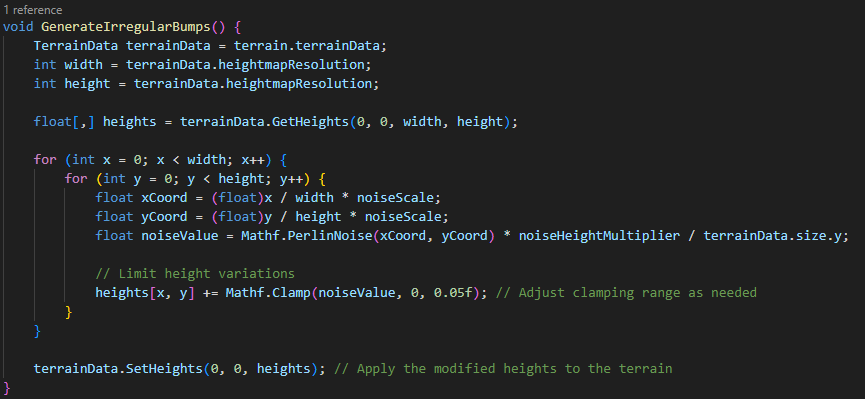
\includegraphics[width=\columnwidth]{figures/irregular_bumps_code.png}}
\caption{Irregular bumps code.}
    \label{fig:irregular_bumps_code}
\end{figure}

\begin{figure}[H]
\centerline{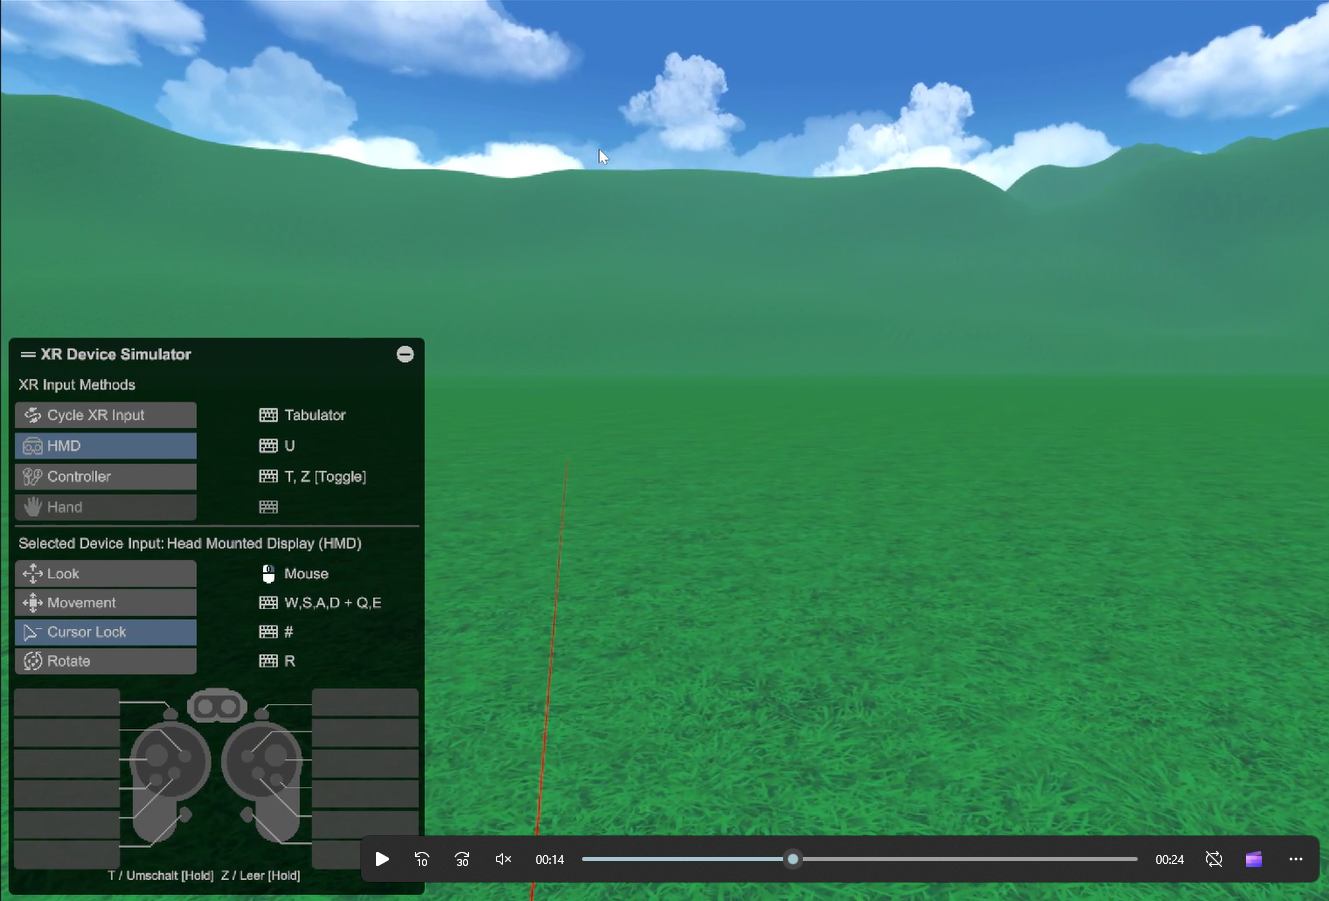
\includegraphics[width=\columnwidth]{figures/flat_terrain.png}}
\caption{Flat terrain.}
    \label{fig:flat_terrain}
\end{figure}

\begin{figure}[H]
\centerline{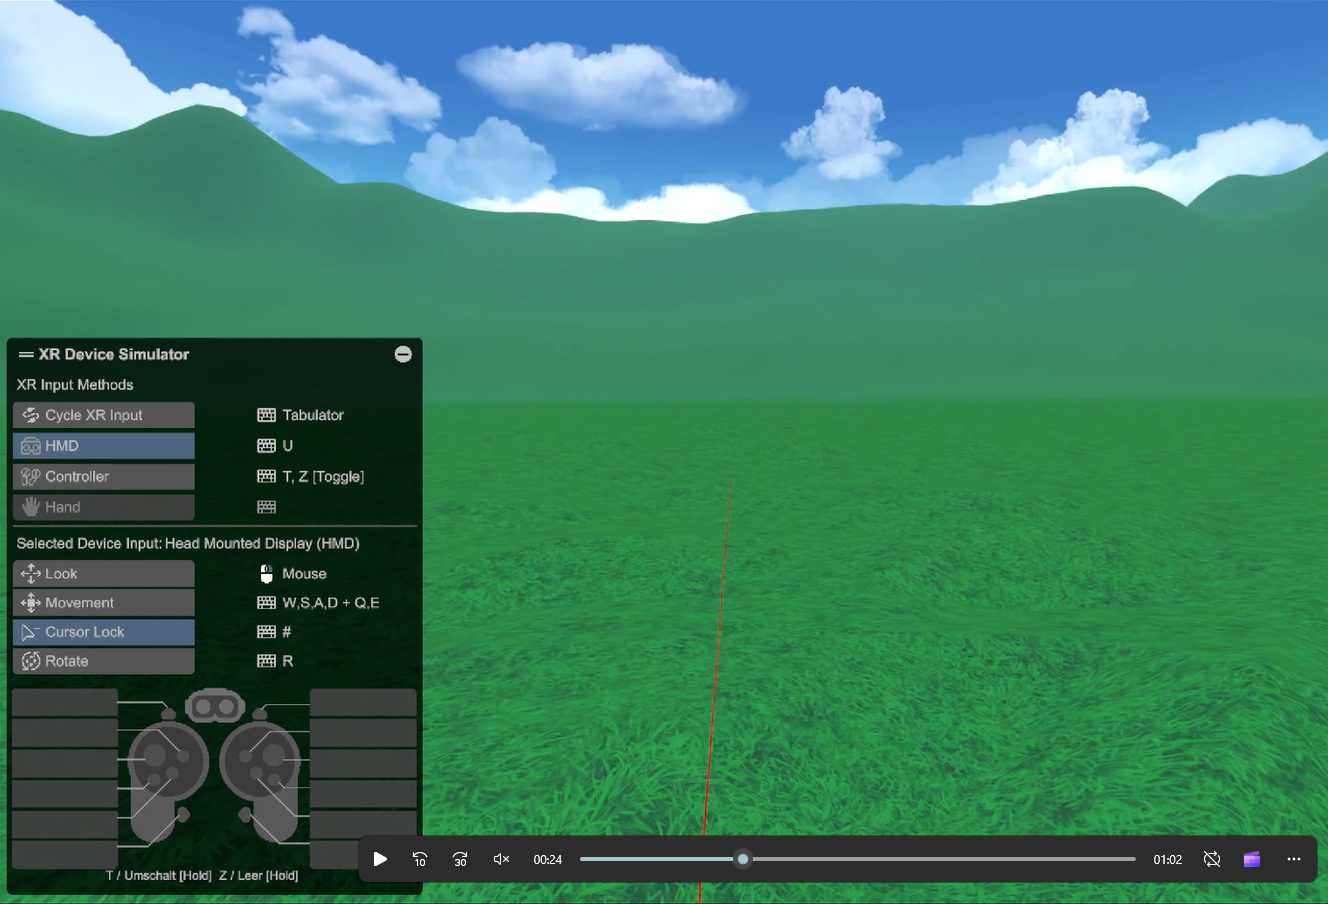
\includegraphics[width=\columnwidth]{figures/bumpy_terrain.png}}
\caption{Bumpy terrain.}
    \label{fig:bumpy_terrain}
\end{figure}

\begin{figure}[H]
\centerline{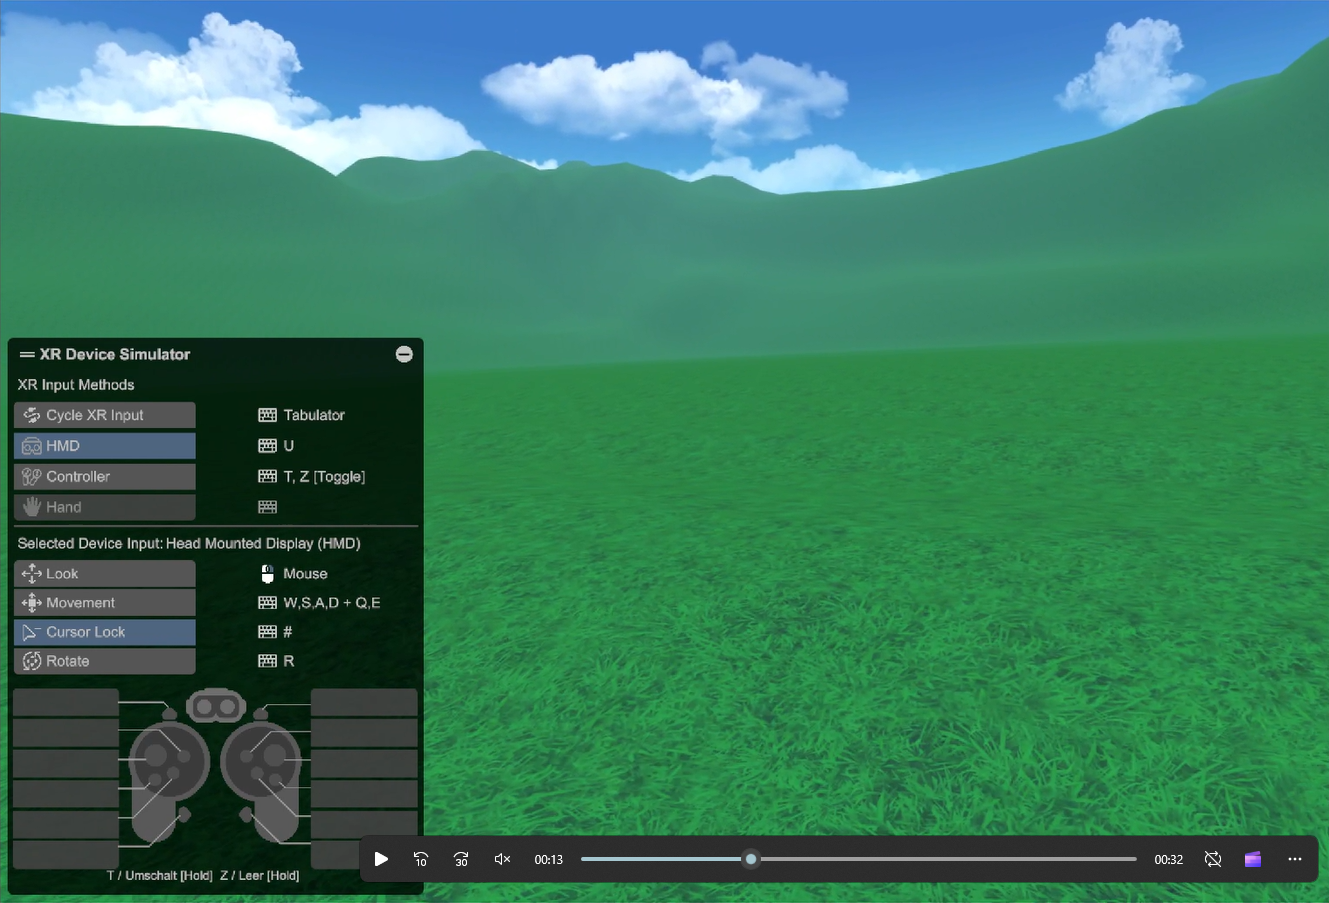
\includegraphics[width=\columnwidth]{figures/regular_terrain.png}}
\caption{Terrain with regular bumps.}
    \label{fig:regular_terrain}
\end{figure}

\subsection{Head Oscillation Simulation}
\subsubsection{Research on Head Oscillations}
Initially, the data used for head movements were taken from the [\cite{translational_motion}] research paper. These data were obtained during outdoor shots, not in a virtual environment. We quickly realized that the movements obtained did not render well in the virtual environment. We therefore chose another research paper, [\cite{trigger_walking}], as the basis for our head oscillations. In this paper, data were taken while the subject was in the virtual environment.

\subsubsection{Implementation}
To implement the head movements, we used Unity Engine's "Animator" module. With the help of curves, we were able to fine-tune head oscillations during the simulation. Two types of animation were implemented: one for walking and one for running. Switching from one to the other is done using Boolean variables, managed in the code and updated as the user moves. Figures \ref{fig:run_curves} and \ref{fig:walk_curves} show head movements in all three spatial directions. Figure \ref{fig:animator} shows the relationships between states and the variables that allow you to move from one state to another.

\begin{figure}[H]
\centerline{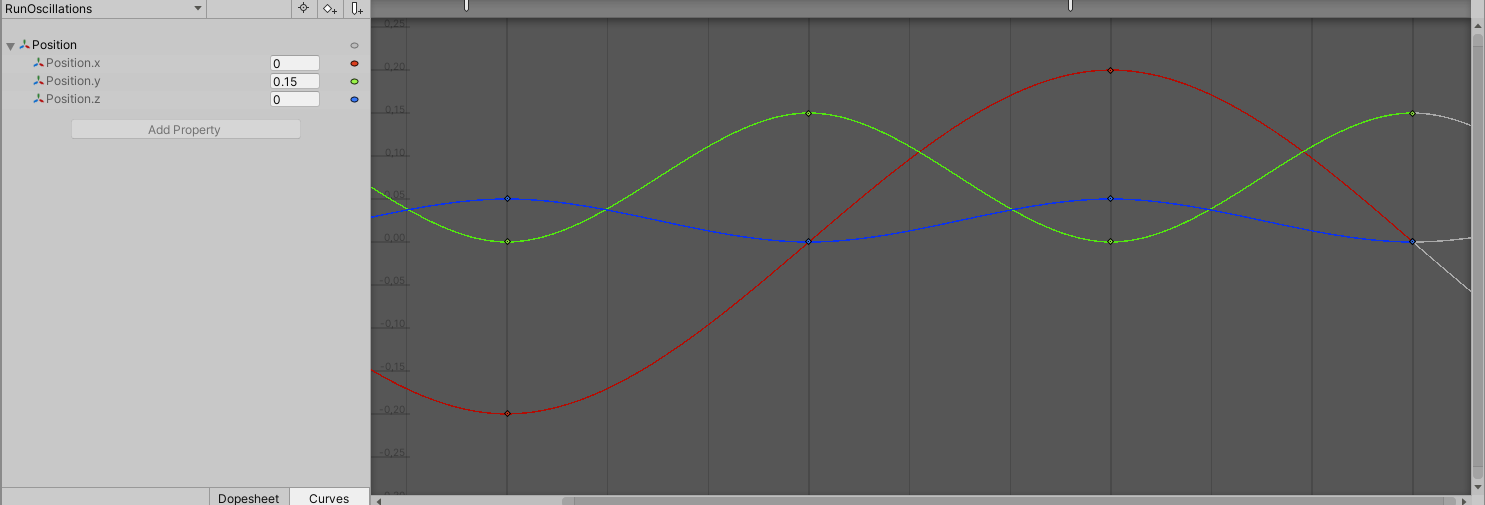
\includegraphics[width=\columnwidth]{figures/run_curves.png}}
\caption{Curves for the running animation.}
    \label{fig:run_curves}
\end{figure}

\begin{figure}[H]
\centerline{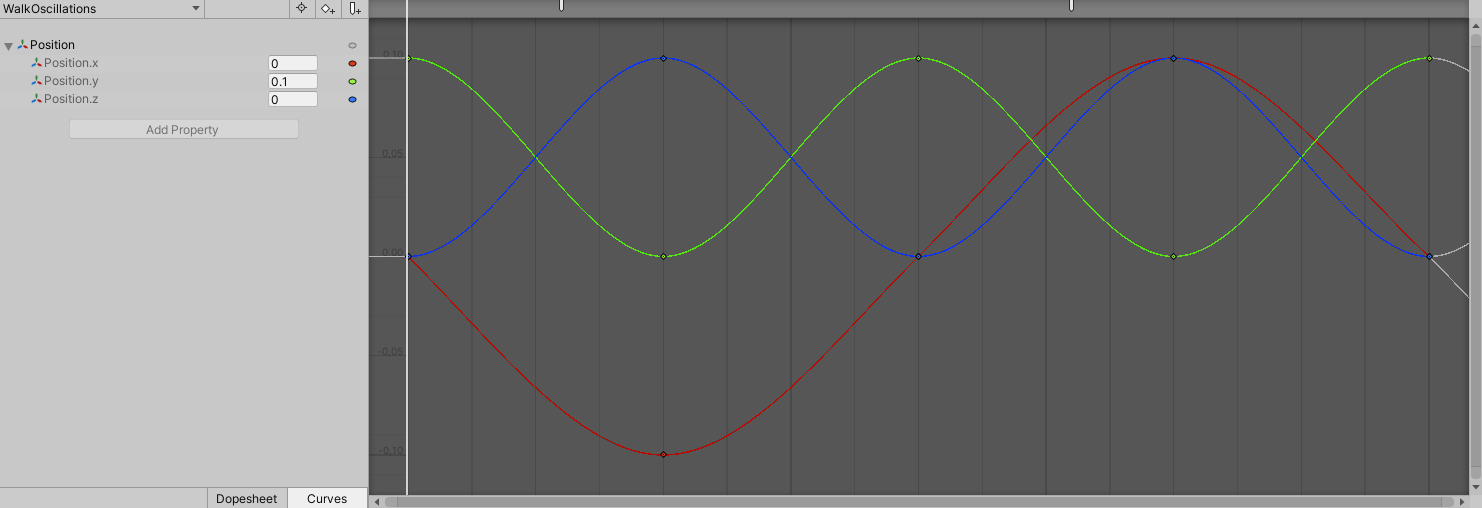
\includegraphics[width=\columnwidth]{figures/walk_curves.png}}
\caption{Curves for the walking animation.}
    \label{fig:walk_curves}
\end{figure}

\begin{figure}[H]
\centerline{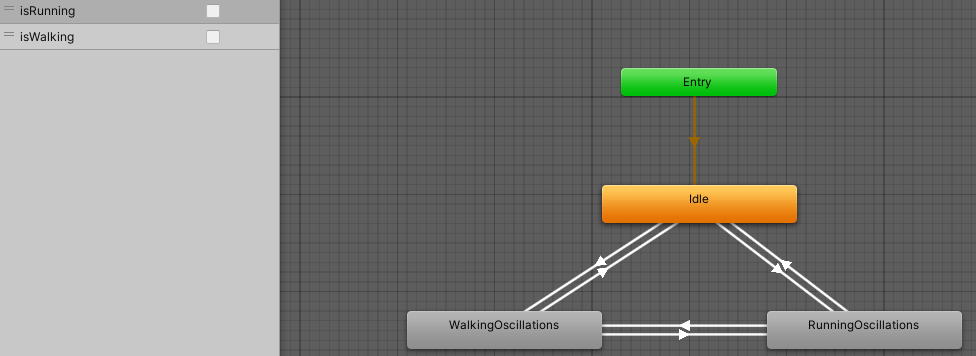
\includegraphics[width=\columnwidth]{figures/animator.png}}
\caption{Links between the different states.}
    \label{fig:animator}
\end{figure}

\subsection{Additional Features}
\subsubsection{Step Sounds}
In the [\cite{walking_vibe}] research paper, it was shown that the presence of footsteps when the user is moving contributes to the reduction of cybersickness. That is why we added this feature, with the option of activating it or not during the simulation. To do this, we searched for an extract of the sound of footsteps on grass in WAV format. We then modified it to the desired duration and applied it to certain events in our animation using a function in our script. Synchronization with head movements was easily achieved using the "Animator" tool.

\subsubsection{Real-Time Monitoring}
To monitor changes in the user's condition in real time, we chose to use Fast Motion Sickness scales [\cite{course}]. There are 7 comfort levels, ranging from 0 (very uncomfortable) to 6 (very comfortable). These appear at given intervals, adjustable from the script. To retrieve test data, a file bearing the scene name is created, and each test result is written to it. These are hidden at the start of the simulation and only appear during the tests. They are placed in a fixed position in the background and appear in front of the user while his or her movements are deactivated.

\begin{figure}[H]
\centerline{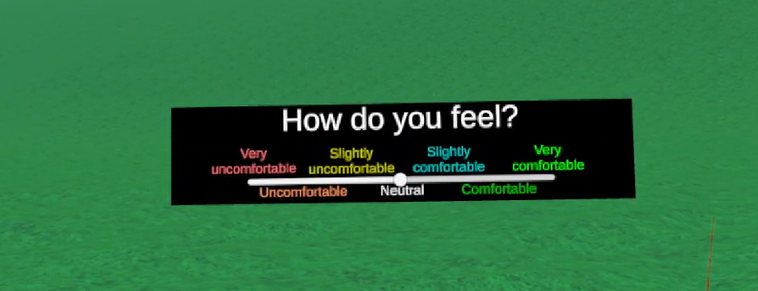
\includegraphics[width=\columnwidth]{figures/test.png}}
\caption{FMS test.}
    \label{fig:test}
\end{figure}

\begin{figure}[H]
\centerline{
\includegraphics[width=\columnwidth]{figures/tests_result.png}}
\caption{One line of a text file containing test results.}
    \label{fig:tests_result}
\end{figure}

\section{Final Product Description}
\label{sec:product}
\subsection{Application overview}
The final simulation therefore has the following elements:
\begin{itemize}[label=\textbullet]
    \item Three different virtual environments,
    \item The ability to activate head oscillations,
    \item The ability to activate footsteps sounds,
    \item Visual comfort tests launched at regular intervals,
    \item The results of these tests are retrieved in a text file for analysis.
\end{itemize}
In addition, the duration of the simulation can also be set from within the script.

\subsection{User controls}
The controls are as follows:
\begin{itemize}[label=\textbullet]
    \item Walk: right OR left trigger button
    \item Run: right AND left trigger button
    \item Increase slider value during test: right trigger button
    \item Decrease slider value during test: left trigger button
    \item Validate test: A button
    \item Activate/deactivate oscillations: right grip button
    \item Activate/deactivate footstep sound during oscillations: left grip button (note: footstep sound can only be heard when oscillations are activated)
\end{itemize}
See figure \ref{fig:quest_controls} for controls.

\begin{figure}[H]
\centerline{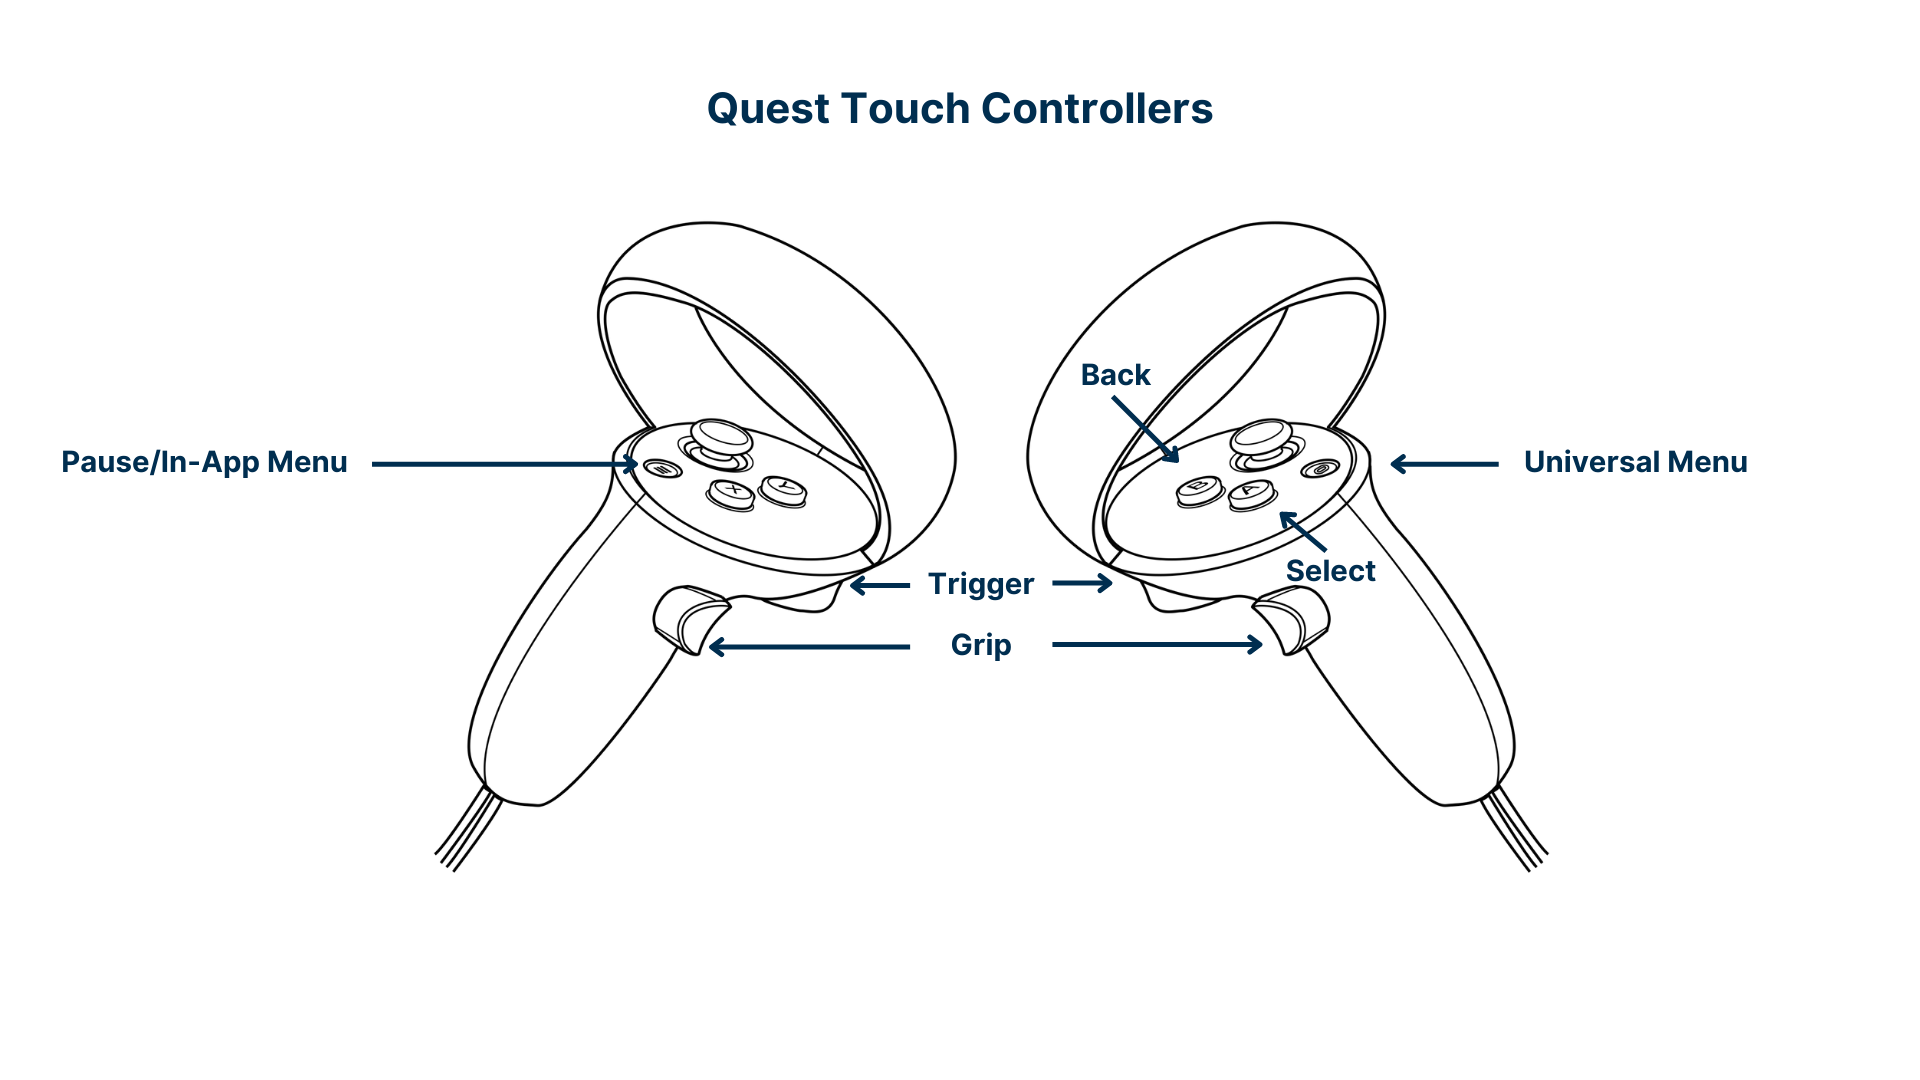
\includegraphics[width=\columnwidth]{figures/quest_controls.png}}
\caption{Quest touch controllers.}
    \label{fig:quest_controls}
\end{figure}

\section{Conclusion}
\label{sec:conclusion}
The aim of this project was to create a versatile simulation to measure the impact of head oscillations on user comfort in virtual reality environments. By implementing three distinct virtual environments - a flat terrain, a terrain with regular bumps and a terrain with noise-generated bumps - we provided a comprehensive basis for future tests and studies.

Key features such as the ability to activate or deactivate head oscillations, the integration of footsteps and real-time monitoring of user discomfort using Fast Motion Sickness scales have been implemented. These features will provide a detailed understanding of how to enhance the virtual reality user experience.

The ability to capture and analyze user comfort data in real time provides valuable information that can be used to refine and improve virtual reality applications in a variety of fields, including medical, gaming and training simulations. The modular design of the simulation allows it to be adapted and extended for future research and development. I look forward to learning about these and following the various studies that may result.

In conclusion, this project has not only enabled me to develop a good tool for research in virtual reality, but it has also enabled me to learn many new concepts. Whether it is handling the Unity Engine or understanding the principles of virtual reality, this new knowledge will certainly benefit me.

\begin{acks}
I would like to express my sincere gratitude to Dr. Jean-Luc Lugrin, my supervisor, for his invaluable help, advice and support throughout this project. His expertise was crucial to the success of this work. Thank you for your continuous guidance and encouragement.
\end{acks}

\listoffigures

\printbibliography

\end{document}

